\begin{appendices}
%\section*{Bijlage A}
%\addcontentsline{toc}{section}{Bijlage A}  

\newpage

\begin{landscape}
\section*{A: OSLO ontology}
\addcontentsline{toc}{section}{A: OSLO ontology}
\label{appendix:oslo:ontology}
    \begin{figure}[H]
    \centering
    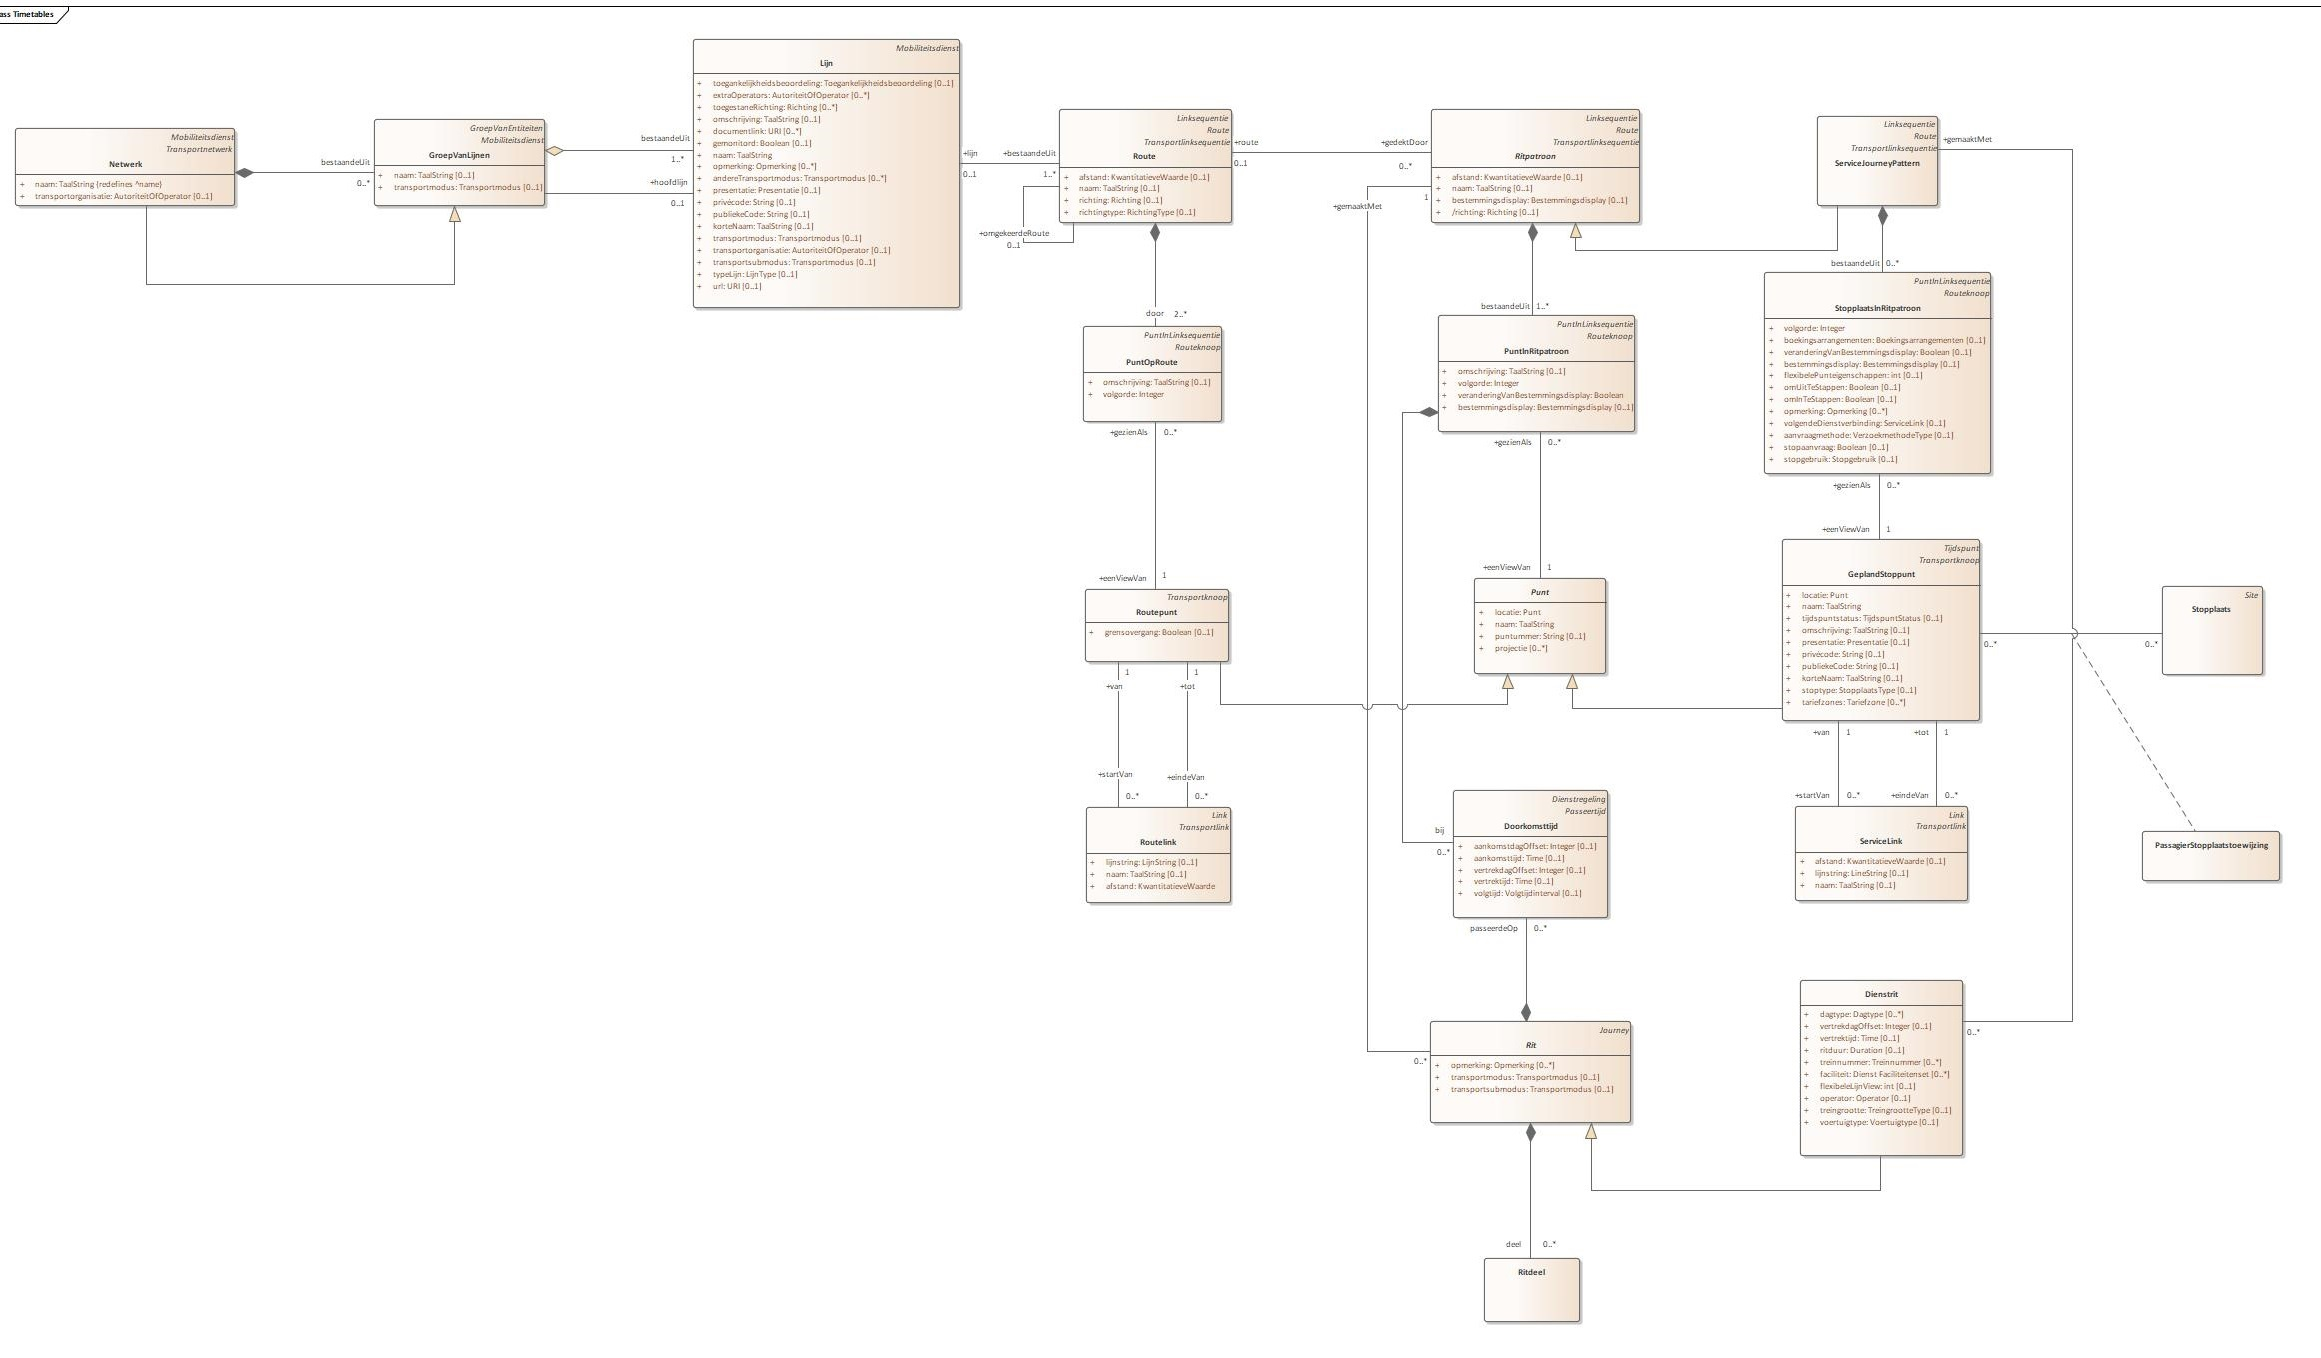
\includegraphics[width=1.4\textwidth]{images/overview.jpg}
    \caption{A small overview of the most important classes in the OSLO Mobility: timetable and route planning algorithm. }
    \tiny For a complete overview, go to \url{https://data.vlaanderen.be/doc/applicatieprofiel/mobiliteit/dienstregeling-en-planning/tijdstabellen/#introduction}
    \label{fig:appendix:Ontology:oslo:overview}
\end{figure}
\end{landscape}


\section*{B: Reference resolver}
\addcontentsline{toc}{section}{B: References resolver}
\begin{listing}[H]
\inputminted[frame=single,linenos,breaklines]{TypeScript}{code/resolve_entities.tex}
\caption{Code to create a graph using the references found in an entity.}
\label{code:resolve}
\end{listing}

\section*{C: Shacl validator}
\addcontentsline{toc}{section}{C: Shacl validator}
\begin{listing}[H]
\inputminted[frame=single,linenos,breaklines]{TypeScript}{code/shacl.ts}
\caption{Code to validate a merged entity}
\label{code:shacl:validator}
\end{listing}

\section*{D: Load}
\addcontentsline{toc}{section}{D: load server}
\begin{figure}[H]
    \centering
    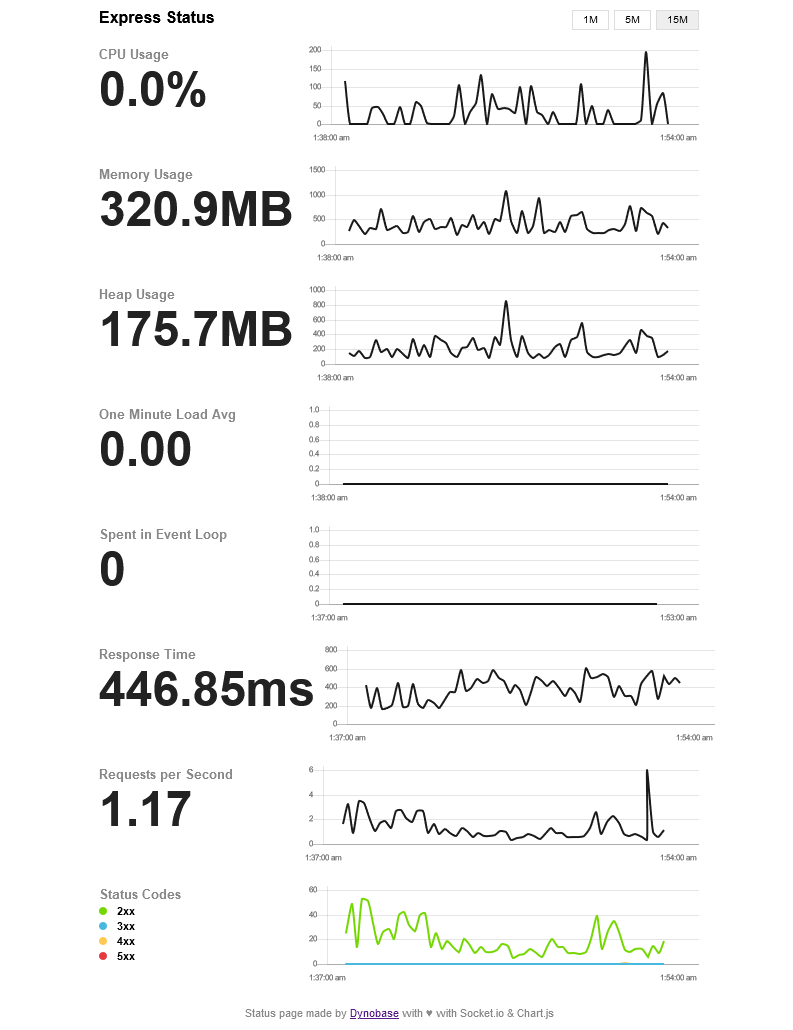
\includegraphics[width=\textwidth]{images/load.png}
    \caption{Multiple metrics indicating load on the server. }
    \label{fig:load}
\end{figure}

\section*{E: Gitlab structure}
\addcontentsline{toc}{section}{E: Gitlab structure}
The thesis resulted in some Gitlab repos. A short description of all these repos you can find below.
\begin{enumerate}
    \item gtfs 2 transmodel ontology: Data parser. this takes an \glsxtrshort{gtfs}-feed and converts to the oslo ontology
    \item gtfs-downloader: Downloads and manages of \glsxtrshort{gtfs} feeds.
    \item gtfs-serve-large: Old version of parser before we swapped it out with our own version.
    \item raptor: This is the raptor implementation and demo.
    \item thesis latex: Latex code of the thesis also contains all images and tikz code.
    \item ts-array-utils: A helper library created by the same author of the raptor implementation. Some changes were made to support newer Node.js versions.
\end{enumerate}

\section*{F: Route list}
\addcontentsline{toc}{section}{F: Route list}
\label{app:routelist}
The list based on personal trajectories:
\begin{itemize}% done
    \item Ostende-Bruges 
    \item Koksijde-Ghent % done
    \item Koksijde-oostende % done
    \item Ostende-Ghent % done
    \item Ostend - Eupen (longest track in Belgium)
    \item Ghent-De panne (plopsaland) % done
    \item Ostende-Waver (Walibi) % done
    \item Ghent-Knokke % done
    \item Ghent-Antwerp central %done
\end{itemize}
The list with popular trajectories:
\begin{itemize}
    \item Antwerpen - Gent
    \item Antwerpen - Hasselt
    \item Antwerpen - Leuven
    \item Antwerpen - Lommel
    \item Antwerpen - Mechelen
    \item Antwerpen - Mol
    \item Antwerpen - Turnhout
    \item Brussel - Antwerpen
    \item Brussel - Gent
    \item Brussel - Leuven
    \item Brussel - Brussels Airport - Zaventem
    \item Gent - Brugge 
\end{itemize}

\end{appendices}